\documentclass[final]{beamer}
\usepackage[orientation=portrait,size=a1,scale=1.18]{beamerposter}
\geometry{hmargin=1.5cm,vmargin=0cm}
\usepackage[utf8]{inputenc}
\linespread{1.04}

% Custom theme
\usetheme{sharelatex}
\definecolor{primary}{RGB}{160,32,60}

% Packages
\usepackage{amsmath,amssymb}
\usepackage{graphicx}
\usepackage{tikz}
\usepackage{multicol}
\usepackage{xcolor}
\usepackage{enumitem}
\usepackage{subcaption} % in preamble
\setlist[itemize]{leftmargin=1.5em, itemsep=0.35em, parsep=0pt, topsep=0.2em}
\setlength{\columnsep}{2cm}
\usepackage[backend=bibtex, style=numeric, sorting=none, maxnames=2, minnames=1]{biblatex}
\AtBeginBibliography{
  \fontsize{16.15}{7}\selectfont
  \setlength{\itemsep}{0pt}
  \setlength{\parskip}{0pt}
}
\addbibresource{bibliography.bib}


% ── Title block ───────────────────────────────────────────────────────────────
\title[Reinforcement Learning -- CentraleSup\'elec]{%
  Sneakie : Learning to play the snake game in all its forms}
\author{Fotios Kapotos, Adonis Jamal, Jean-Vincent Martini}
\institute[CentraleSup\'elec]{CentraleSup\'elec}
\date{March 2026}

% =============================================================================
\begin{document}
\begin{frame}[t] 
\vskip0.1cm
\begin{multicols}{2}

% ── Block 1 : The Snake Game ──────────────────────────────────────────────────
\begin{block}{1. The Snake Game}

\begin{figure}[h]
    \centering
    \begin{subfigure}{0.48\linewidth}
        \centering
        \includegraphics[width=\linewidth]{img/snake_simple_early.png}
        \caption{Early version}
    \end{subfigure}
    \hfill
    \begin{subfigure}{0.48\linewidth}
        \centering
        \includegraphics[width=\linewidth]{img/snake_simple_late.png}
        \caption{Later version}
    \end{subfigure}
    \caption{Comparison of the snake agent over training.}
    \label{fig:snake_comparison}
\end{figure}

\textbf{MLP agent} : 15-dim hand-crafted state vector:
\begin{itemize}
  \item Danger flags (straight, left, right) + current direction (one-hot)
  \item Bearing to nearest food and poison (4 binary flags each)
  \item Food location is \emph{given explicitly}: agent never needs to search the grid
\end{itemize}

\begin{figure}[h]
  \centering
  \begin{subfigure}{0.48\linewidth}
    \centering
    \includegraphics[width=\linewidth]{img/MLP rewards.png}
    \caption{Baseline vs.\ step penalty vs.\ distance shaping}
  \end{subfigure}
  \hfill
  \begin{subfigure}{0.48\linewidth}
    \centering
    \includegraphics[width=\linewidth]{img/reward magnitude_scaling.png}
    \caption{Effect of reward magnitude scaling}
  \end{subfigure}
  \caption{MLP agent snake length over training (5\,000 episodes, $16\!\times\!16$ grid).}
\end{figure}

\textbf{CNN agent} : egocentric window $(6\!\times\!k\!\times\!k)$ centered on the head:
\begin{itemize}
  \item Channels: body, head, food, obstacles
  \item Observation is a \emph{local crop} around the snake head (e.g.\ $k=9$ or $11$), updated at each step
  \item Removes global search: relevant information is spatially \emph{localized} by construction
  \item \textbf{Inductive bias:} translation invariance + locality match the control problem (decisions depend on nearby hazards and targets)
\end{itemize}
\textbf{Full-CNN agent} : global grid observation $(C\!\times\!H\!\times\!W)$ over the whole board:
\begin{itemize}
  \item Channels typically encode body, head, food, and obstacles over the full map
  \item Observation is the \emph{entire environment} at each step
  \item Preserves complete spatial information, including long-range structure and global planning cues
  \item \textbf{Inductive bias:} convolution exploits spatial regularities on the grid, but the agent must still learn which regions are relevant for decision-making
\end{itemize}

\begin{figure}[h]
    \centering
    \includegraphics[width=0.7\linewidth]{img/Ergovsfull.png}
    \caption{Comparison between full-grid CNN and egocentric CNN observations.}
    \label{fig:egovfull}
\end{figure}
\end{block}


% ── Block 2 : The Long Snake Problem ─────────────────────────────────────────
\begin{block}{2. The Long Snake Problem}

\begin{figure}[h]
    \centering
    \includegraphics[width=0.3\linewidth]{img/Long snake problem.png}
    \caption{Snake is trapped}
    \label{fig:snaketrapped}
\end{figure}

\small
\textbf{Issue:} early policy = greedy food chasing.  
At large length, this leads to \emph{self-trapping} (no global planning).
\textbf{Conflict:} short-term reward (food) vs long-term survival.


\textbf{Fix:} add a \emph{repulsion reward} from the body  
$\rightarrow$ encourages spacing and prevents collapse.

\end{block}
\columnbreak


% ── Block 3 : Hard Mode Environment ──────────────────────────────────────────
\begin{block}{5. Tuning Agents specifically for hard mode}
\begin{figure}[h]
    \centering
    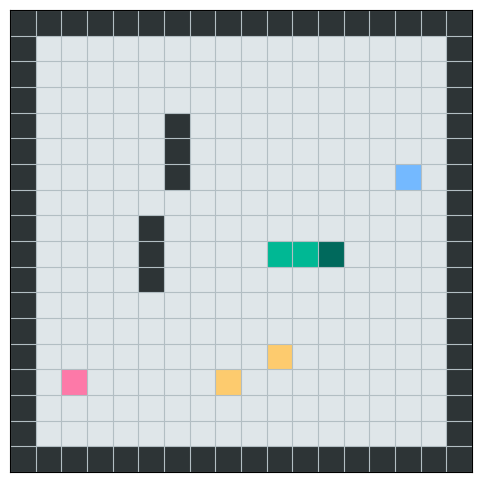
\includegraphics[width=0.5\linewidth]{img/map_hard.png}
    \caption{Hard environment: gold, silver, and poison food alongside static obstacles on a $16\!\times\!16$ grid}
    \label{fig:map_hard}
\end{figure}

% \begin{itemize}
%   \item \textbf{Gold food} ($+5$): primary target; respawns immediately after eating
%   \item \textbf{Silver food} ($+0.5$): secondary target; worth pursuing when gold is far
%   \item \textbf{Poison food}: shrinks snake by 2 segments; must be actively avoided
%   \item \textbf{Static obstacles}: fixed 3-cell walls placed at episode reset; lethal on contact
%   \item \textbf{Dynamic obstacles}: 3-cell walls bouncing back and forth within a fixed range; lethal even if the wall \emph{moves into} a stationary snake
% \end{itemize}

\end{block}


% ── Block 4 : Strategies ──────────────────────────────────────────────────────
\begin{block}{4. How adaptable are the agents ? }

\textbf{MLP agent:} requires manual redesign of the state vector  
(danger $\rightarrow$ poison/obstacles, food $\rightarrow$ merged signal).  
Performs well in simple settings, but struggles with \emph{dynamic elements}  
(e.g.\ moving obstacles), often getting stuck in \emph{behavioral loops}.

\vspace{0.3em}
\textbf{CNN agent:} directly processes spatial observations.  
Adapts naturally to new objects without feature engineering.  
More robust to complexity and dynamics, achieving \emph{higher performance}  
and fewer failure modes.

\begin{center}
\small
\begin{tabular}{lcccc}
\textbf{Agent} & \textbf{Mean length} & \textbf{Mean reward} & \textbf{Mean foods} & \textbf{Loop rate} \\
\hline
MLP (static hard)   & 13.2 & 10.8 & 10.2 & 0.05 \\
MLP (moving obs.)   &  9.1 &  6.7 &  6.4 & 0.27 \\
CNN (static hard)   & 15.6 & 12.9 & 12.5 & 0.02 \\
CNN (moving obs.)   & 14.8 & 11.7 & 11.3 & 0.08 \\
\end{tabular}
\end{center}

\end{block}

% % ── Block 5 : Results ─────────────────────────────────────────────────────────
\begin{block}{5. Agents specifically for hard mode}
\textbf{State \& architecture}
\begin{itemize}
  \item \textbf{Frame stacking ($n\!=\!4$):} stacks the last 4 grid observations into a $(4C\!\times\!H\!\times\!W)$ tensor; encodes obstacle \emph{velocity} and near-miss dynamics, converting a partially-observable environment into an approximately Markovian state
  \item \textbf{Dueling and Double QDN:} shared convolutional trunk splits into a state-value head $V(s)$ and an advantage head $A(s,a)$; $Q = V + (A - \bar{A})$; faster convergence in states where survival matters more than which food to chase
\end{itemize}

\textbf{Reward engineering}
\begin{itemize}
  \item \textbf{Distance shaping:} $r_t \mathrel{+}= \lambda\,(d_{t-1} - d_t)$ toward nearest gold/silver; 
  \item \textbf{Body-proximity shaping:} $r_t \mathrel{+}= \mu\,(b_t - b_{t-1})$ where $b_t$ is distance to nearest body 
  \item \textbf{Step penalty ($-0.01$/step):} penalises stalling
\end{itemize}

\begin{figure}[h]
    \centering
    \includegraphics[width=0.7\linewidth]{img/Hard_cnn_mlp.png}
    \caption{CNN vs MLP Agents comparison in hard mode}
    \label{fig:example}
\end{figure}
\end{block}

\begin{block}{6. Final performance}
  \begin{figure}[h]
    \centering
    \includegraphics[width=0.4\linewidth]{img/final snakie.png}
    \caption{Final state of the snake agent}
    \label{fig:final}
\end{figure}
\end{block}


\end{multicols}
\end{frame}
\end{document}
